\documentclass[14pt]{extarticle}

\usepackage[]{cite}
\usepackage{cmap}
\usepackage[T2A]{fontenc}
\usepackage[utf8]{inputenc}
\usepackage[english, russian]{babel}

% \usepackage{jmlda}
\newcommand{\hdir}{.}
\usepackage{amsmath, amsfonts,amssymb,mathrsfs}
\usepackage{graphicx}
\usepackage{minted}
\usepackage{hyperref}
\usepackage{mathtools}
\usepackage{tocloft}
\usepackage[linesnumbered,boxed]{algorithm2e}
% \usepackage{algorithm}
% \usepackage{algpseudocode}
% \usepackage[usenames]{color}
% \usepackage{colortbl}


\usepackage{graphicx, epsfig}
\usepackage{subfig}
\usepackage{color}

\usepackage{wrapfig}
\usepackage{float}
\usepackage{subfloat}
\usepackage{caption}
\usepackage{multirow}
\usepackage{pdfpages}


\newtheorem{theorem}{Теорема}
\newtheorem{lemma}[theorem]{Лемма}
\newtheorem{definition}{Определение}
\newtheorem{remark}{Замечание}
\newenvironment{Proof} % имя окружения
    {\par\noindent{\bf Доказательство.}} % команды для \begin
    {\hfill$\scriptstyle\blacksquare$} % команды для \end

\DeclareMathOperator*{\argmax}{arg\,max}
\DeclareMathOperator*{\argmin}{arg\,min}
\newcommand{\Domain}{\mathcal{D}}
\newcommand{\supp}{\mathrm{supp}}
\newcommand{\diag}{\mathrm{diag}}
\newcommand{\bfw}{\mathbf{w}}
\newcommand{\bfv}{\mathbf{v}}
\newcommand{\bfx}{\mathbf{x}}
\newcommand{\bfz}{\mathbf{z}}
\newcommand{\bfX}{\mathbf{X}}
\newcommand{\bfy}{\mathbf{y}}
\newcommand{\bfb}{\mathbf{b}}
\newcommand{\bbr}{\mathbb{R}}
\newcommand{\cala}{\mathcal{A}}
\newcommand{\bsigma}{\boldsymbol\Sigma}
\newcommand{\bvareps}{\boldsymbol{\varepsilon}}
\newcommand{\expectation}{\mathbb{E}}
\newcommand{\ceil}[1]{\lceil #1 \rceil}
\newcommand{\btheta}{\boldsymbol{\theta}}


\def\BibAuthor#1{\ruseng{\textit{#1}}}
\def\BibTitle#1{\ruseng{\textrm{#1}}}
\def\BibJournal#1{\ruseng{\textrm{#1}}{\textsl{#1}}}
\def\BibUrl#1{{\small\url{#1}}}
\def\BibHttp#1{{\small\url{http://#1}}}
\def\BibFtp#1{{\small\url{ftp://#1}}}
\def\BibDoi#1{doi:~{\small\url{http://dx.doi.org/#1}}}
\def\typeBibItem{\small\sloppy}


\textheight=22cm % высота текста
\textwidth=16cm % ширина текста
\oddsidemargin=0pt % отступ от левого края
\topmargin=-1.5cm % отступ от верхнего края
\parindent=24pt % абзацный отступ
\parskip=5pt % интервал между абзацами
\tolerance=2000 % терпимость к "жидким" строкам
\flushbottom % выравнивание высоты страниц

\begin{document}
\thispagestyle{empty}

\begin{center}
    \bf\Large
		Оценка качества декомпозиции данных fMRI в домене синограмм для различных аффинных преобразований данных. \\[10mm]
	\rm\large
        Шокоров Вячеслав Александрович\\[10mm]
\end{center}

\section{Мотивация}

Тензорная аппроксимация имеет решающее значение для современных численных приложений. Существует несколько методов, но нет четкого понимания того, как они сравниваются с точки зрения качества. В этой работе исследуется проблема влияния различных аффинных преобразований отдельных изображений на качество декомпозиции полного временного ряда видео. Эксперимент проводится на данных fMRI и, исследуется устойчивость декомпозиции в домене синограмм к различным смещениям.
 \\

%данные поля заполняются редакцией журнала
% \doi{10.21469/22233792}
% \receivedRus{01.01.2017}
% \receivedEng{January 01, 2017}

% \maketitle

% \cftchapterprecistoc




\section{Введение}

\begin{figure}[h]
        \centering
        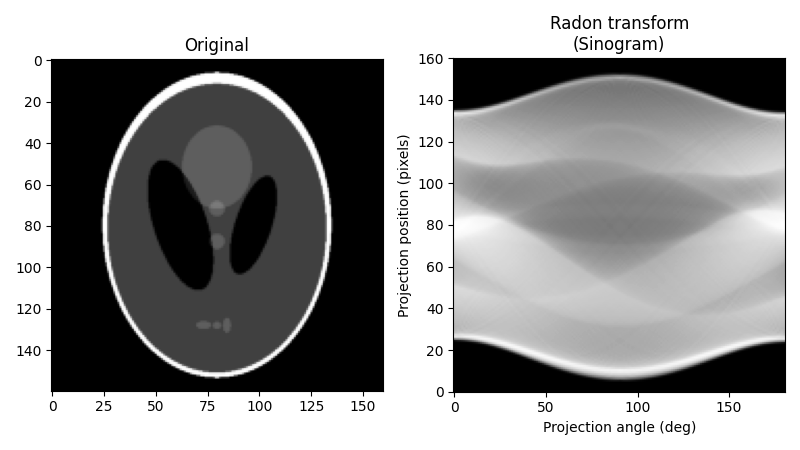
\includegraphics[width=0.8\textwidth]{orig-sinogram.png}
        
        \caption{Пример изображения и его синограммы.}
        \label{fig_1}
\end{figure}

Медицинское исследование, компьютерная томография представляет собой быстро вращающийся сканер, который получает изображения называемые синограммами (см. \ref{fig_1}). Для того, чтобы получить из синограммы изображение (срез) объекта применяется преобразование Радона. Это интегральное преобразование функции многих переменных, родственное преобразованию Фурье. 

Рассмотрим наиболее простой случай преобразования Радона, случай функции двух переменных.
Пусть $f(x,y)$ функция двух действительных переменных, определённая на всей плоскости и достаточно быстро убывающая на бесконечности (так, чтобы соответствующие несобственные интегралы сходились). Тогда преобразованием Радона функции $f(x,y)$ называется функция

$$ R(s,\alpha ) = \int \limits _{-\infty }^{\infty }f(s\cos \alpha -z\sin \alpha ,s\sin \alpha +z\cos \alpha )dz$$ 

Преобразование Радона имеет простой геометрический смысл — это интеграл от функции вдоль прямой, перпендикулярной вектору $\vec{n}=(\cos \alpha ,\sin \alpha )$ и проходящей на расстоянии $s$ (измеренного вдоль вектора $\vec{n}$, с соответствующим знаком) от начала координат.

\section{Постановка задачи декомпозиции (HOSVD)}

Пусть $\mathbf{\underline{X}} \in \mathbb{R}^{I \times J \times K}$ - тензор размерности 3, тогда декомпозиция Такера имеет следующий вид:

\begin{equation}
    \label{Tucker_format}
    \mathbf{\underline{X}} \simeq \mathbf{\underline{G}} \times_1 \mathbf{A} \times_2 \mathbf{B} \times_3 \mathbf{C}
\end{equation}

Для метода HOSVD накладываются дополнительные ограничения в виде ортогональности матриц.

Из \eqref{Tucker_format} видно, что если мы случайным образом перемешаем пиксели видео и сделаем декомпозицию Такера, получим $\{\underline{G}', \mathbf{A}', \mathbf{B}', \mathbf{C}'\}$. Тогда можно получить исходные матрицы для неперемешанного видео, сделав соответствующую переиндексацию координат. Для доказательства этого факта достаточно показать, что это утверждение верно при перемешивании 2х случайных пикселей. Случайное перемешивание всех пикселей это композиция нескольких перемешиваний пар пикселей.

Пусть $I, J$ - соответствуют координатам пикселей
\begin{definition}
    Назовем \textit{дисперсией пикселя} $[i, j]$ для набора изображений описаных тензором $\mathbf{\underline{X}} \in \mathbb{R}^{I \times J \times K}$:
    \begin{multline}
        \label{opt_transorm_f}
        S_X(i, j) = \frac{1}{K} \sum_{k=1}^K(X[i, j, k] - \overline{X}[i, j, :])^2 = \\ = \frac{1}{K} \sum_{k=1}^K X^2[i, j, k] - \left (\frac{1}{K} \sum_{k=1}^K X[i, j, k] \right )^2
    \end{multline}
\end{definition}

\section{Вычислительный эксперимент}

Вычислительный эксперимент проводится на томографических рентгеновских данных "dynamic agarose-gel phantom" перфузированного жидким контрастным веществом. Набор данных состоит из 17 последовательных рентгеновских измерений 2D-среза.

\begin{figure}[H]
        \centering
        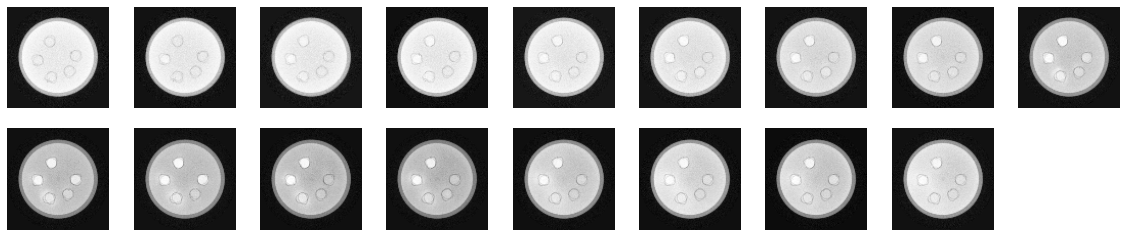
\includegraphics[width=1\textwidth]{all_data.png}
        
        \caption{Реконструированные данные из синограмм. На картинках изображено 17 кадров (2D-срезов) томографических рентгеновских данных "dynamic agarose-gel phantom" перфузированного жидким контрастным веществом.}
        \label{fig_2}
\end{figure}


\begin{figure}[H]
        \centering
        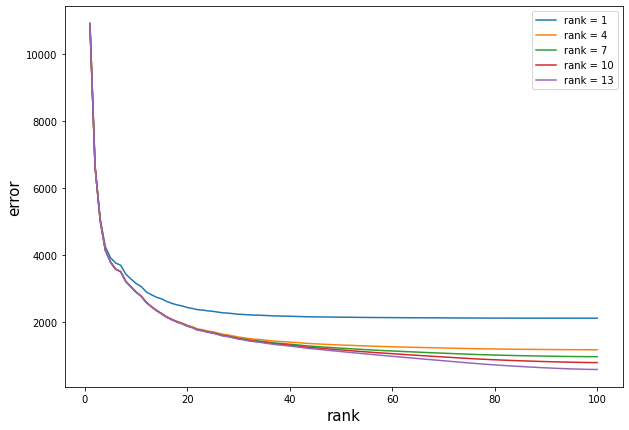
\includegraphics[width=1\textwidth]{exp_1.png}
        
        \caption{Зависимость ошибки аппроксимации тензора от ранга. Видно, что с увеличением сложности и правильно подобранных параметрах модели итоговая ошибка падает. Ошибка считается как норма Фробениуса разности тензора и его аппроксимации.}
        \label{fig_3}
\end{figure}


\begin{figure}[H]
        \centering
        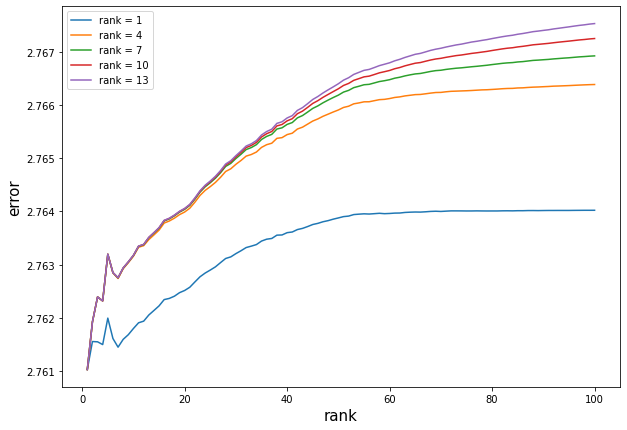
\includegraphics[width=1\textwidth]{exp_2.png}
        
        \caption{Берется набор синограмм изображений, строится аппроксимации тензора, которая переводится обратно в домен изображения с помощью обратного преобразования Радона. Для каждой реконструкции считается ошибка как норма Фробениуса разности тензора и его аппроксимации. Рост ошибки скорее всего связан с тем, что при декомпозиции мы решаем задачу минимизации в евклидовом пространстве матриц:$$\| \mathbf{\underline{X}} - \mathbf{\underline{G}} \times_1 \mathbf{A} \times_2 \mathbf{B} \times_3 \mathbf{C} \| \to \min_{\mathbf{\underline{G}}, \mathbf{A}, \mathbf{B}, \mathbf{C}},$$ А ошибка считается в сопряженном пространстве изображений:
        $$\mathrm{error} = \| \mathbf{\underline{X}} - \underline{R}\left (\mathbf{\underline{G}} \times_1 \mathbf{A} \times_2 \mathbf{B} \times_3 \mathbf{C}\right) \|,$$ где $\underline{R}$ - преобразование Радона примененное к каждому изображению в серии независимо.}
        \label{fig_3}
\end{figure}

\begin{figure}[H]
        \centering
        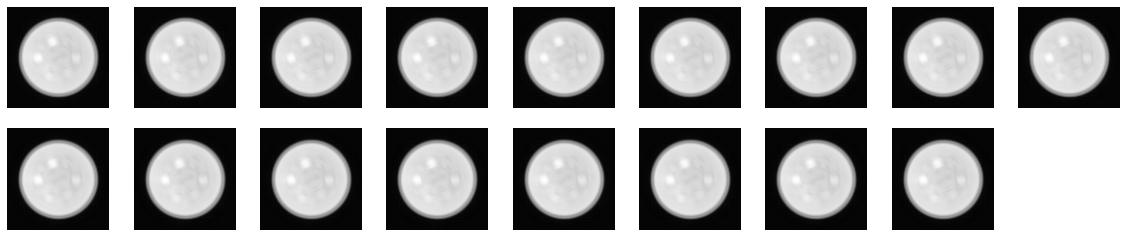
\includegraphics[width=1\textwidth]{exp_3.png}
        
        \caption{Реконструированные изображения из аппроксимации синограмм.}
        \label{fig_5}
\end{figure}

Описание рис. \ref{fig_5}. Ранее было введено определение дисперсии пикселя. На графиках изображено значение ошибки аппроксимации и дисперсии для каждого пикселя для соответствующего размера ранга декомпозиции. Размер аппроксимируемого изображения - $100\times100$, а число кадров - $17$. Поэтому ранг $(100, 100, 15)$ позволяет почти полностью реконструировать изображение. Ранг $(100, 100, 1)$ позволяет хорошо реконструировать общий вид изображения, но не дает возможность учитывать временную зависимость. В таком случае дисперсия пикселя \textbf{сильно коррелирует} с точностью реконструкции изображения после декомпозиции.

\begin{figure}[h]
        \centering
        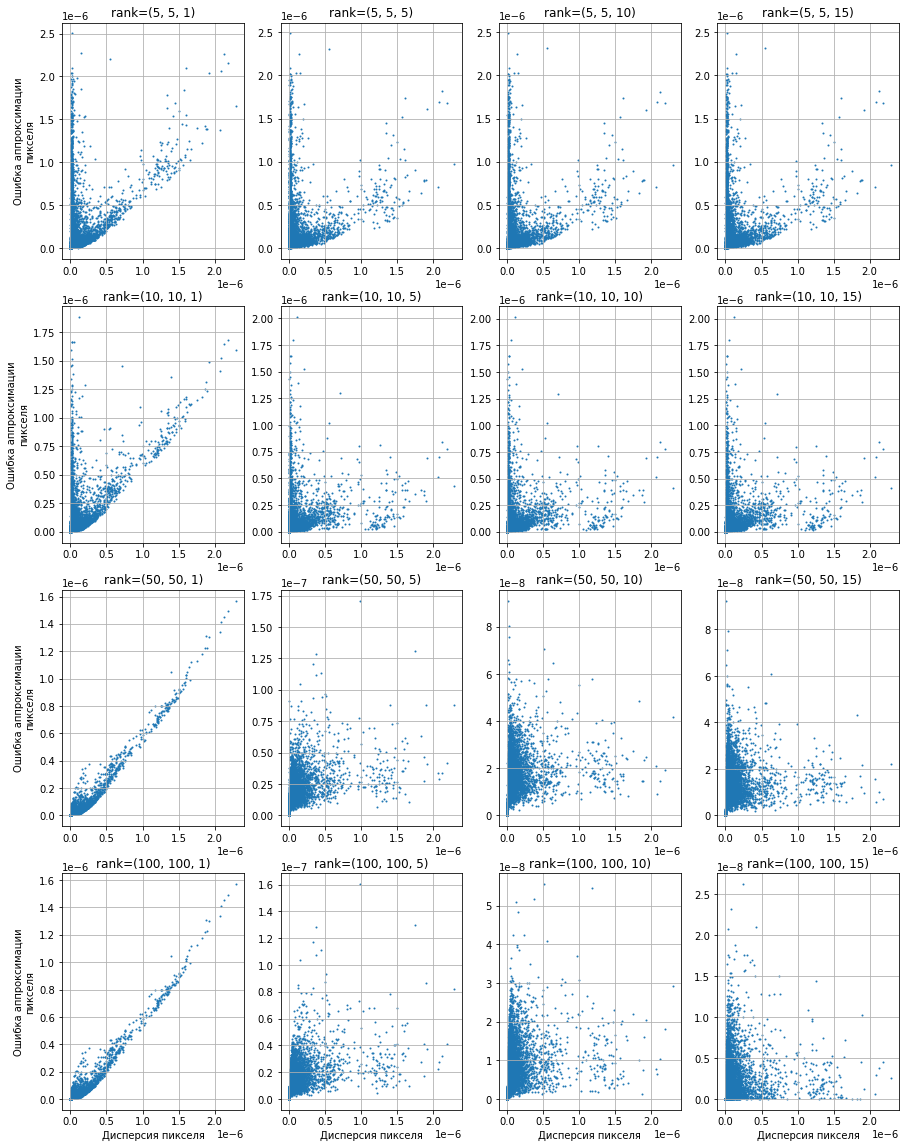
\includegraphics[width=1\textwidth]{exp_4.png}
        
        \caption{}
        \label{fig_5}
\end{figure}

\end{document}